\section{Geradlinige Dreiecks Darstellungen (SLTRs)}

Ausgehend von den konvexen Einbettungen nach Tutte, kann man sich die Frage stellen, unter welchen Vorraussetzungen wir einen planaren Graphen so zeichnen können, dass alle Gebiete Dreiecke umranden. Die Formalisierung dieser Darstellung und erste Folgerungen folgen Nieke Aerts und Stefan Felsner \cite{af13,af15}.

\begin{definition}[SLTR]\label{defsltr}
Eine Zeichnung eines planen Graphen $G$ wird \textit{geradlinige Dreiecks Darstellung}, im weiteren kurz \textit{SLTR} (für die englische Bezeichnung \textit{staight line triangle representation}), genannt falls gilt:
\begin{itemize}
\item[S1] Alle Kanten sind Segmente von Geraden.
\item[S2] Alle Gebiete, inklusive dem Äusseren, sind nicht degenerierte Dreiecke.
\end{itemize}
\end{definition}

\begin{figure}[h]
	\centering
  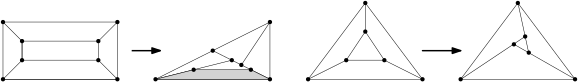
\includegraphics[width=0.9\textwidth]{sltr-example.png}
	\caption{Links einer der beiden 3-zusammenhängenden Graphen auf acht Knoten ohne SLTR und rechts ein Graph mit einer möglichen SLTR.}
\end{figure}

Um die Problemstellung greifbarer zu machen kann man plane Graphen zusammen mit den Aufhängungen $\{a_1,a_2,a_3\}$ betrachten, wobei $\{a_1,a_2,a_3\}$ hier die designierten Ecken des äusseren Gebietes einer möglichen SLTR sind. Einen Graphen zusammen mit einem äusseren Gebiet bzw. festen Aufhängungen als Paar zu behanden ist sinnvoll, weil planare Graphen existieren, von denen manche Einbettungen, SLTRs zulassen, andere jedoch nicht, so wie in Abbildung \ref{10_example} zu sehen. Zumindest für 3-zusammenhängende planare Graphen ist die topologische Einbettung nach der Auswahl der Aufhängungen eindeutig.

\begin{proposition}\cite[Proposition 1.2]{af13}
Sei $G$ ein planer Graph mit den Aufhängungen $\{a_1,a_2,a_3\}$ als äussere Ecken einer SLTR. Weiter gebe es keine inneren Knoten $v$ mit $deg(v) < 3$. Dann ist $G$ intern-3-zusammenhängend.
\end{proposition}

\begin{remark}
Für innere Knoten von Grad 2 in einer SLTR müssen beide angrenzenden Winkel gerade sein. Somit kann man diese Knoten durch eine gerade Kante zwischen ihren Nachbarn ersetzen und den resultierenden Graphen betrachten. Wir werden somit von nun an nur intern-3-zusammenhängende Graphen mit Aufhängungen betrachten, da alle anderen Graphen, die eine SLTR zulassen, auf diese reduziert werden können.
\end{remark}

\begin{figure}[h]
	\centering
  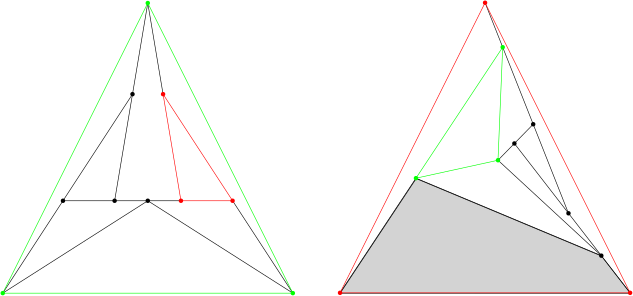
\includegraphics[scale=0.1]{10_example.png}
	\caption{Der kleinste 3-zusammenhängende kombinatorische Graph mit einer Wahl der Aufhängungen die eine SLTR zulässt und einer Auswahl ohne SLTR.}
	\label{10_example}
\end{figure}

Zu den Fragen, welche notwendigen und hinreichenden Bedingungen es für die Existenz von SLTRs gelten und  welche algorithmischen Ansätze man bei der Suche nach einer spezifischen Darstellung verfolgen kann, haben Aerts und Felsner in \cite{af13}, \cite{af13h} und \cite{af15} schon einige Antworten geliefert. Die nächsten zwei Kapitel, werden sich damit beschäftigen. Zuvor müssen in diesem Kapitel noch ein paar notwendige Konzepte eingeführt werden.
